% ============================================================
\chapter{Valeurs Propres et Vecteurs Propres}
\label{ch:vp}
% ============================================================

\section{Exemple motivant}
L'analyse des vibrations d'une structure (pont, b\^atiment) revient \`a trouver les fr\'equences propres, i.e.\ les valeurs propres d'une matrice de rigidit\'e. Pour une matrice $1000\times 1000$, calculer le polyn\^ome caract\'eristique est impraticable : on utilise des m\'ethodes it\'eratives.

\section{Rappels}

\begin{definition}
$\lambda\in\C$ est \textbf{valeur propre} de $A\in\R^{n\times n}$ s'il existe $x\neq 0$ tel que $Ax=\lambda x$. Le vecteur $x$ est un \textbf{vecteur propre} associ\'e. L'ensemble des valeurs propres est le \textbf{spectre} $\sigma(A)$.
\end{definition}

\begin{theoreme}[Propri\'et\'es spectrales]
\begin{itemize}
\item $\sigma(A)\subset\{z : |z|\leq\|A\|\}$ (rayon spectral $\rho(A)\leq\|A\|$).
\item Si $A$ est sym\'etrique r\'eelle, toutes ses valeurs propres sont r\'eelles.
\item Si $A$ est sym\'etrique d\'efinie positive, toutes ses valeurs propres sont strictement positives.
\item Th\'eor\`eme de Gerschgorin\index{Gerschgorin} : $\sigma(A)\subset\bigcup_{i=1}^n D(a_{ii},R_i)$ o\`u $R_i=\sum_{j\neq i}|a_{ij}|$.
\end{itemize}
\end{theoreme}

\section{M\'ethode de la puissance it\'er\'ee}\index{puissance iteree@puissance it\'er\'ee}

\begin{definition}
Pour trouver la valeur propre dominante $\lambda_1$ (celle de plus grand module) et le vecteur propre associ\'e.
\end{definition}

\begin{algorithm}[H]
\caption{Puissance it\'er\'ee}\label{alg:puissance}
\KwEntree{$A\in\R^{n\times n}$, $x^{(0)}$ vecteur initial, tol\'erance $\varepsilon$, $k_{\max}$}
\KwSortie{$\lambda_1$, $x_1$}
\Pour{$k=1,2,\ldots,k_{\max}$}{
  $w\gets Ax^{(k-1)}$\;
  $x^{(k)}\gets w/\|w\|$\;
  $\lambda^{(k)}\gets (x^{(k)})^\top A x^{(k)}$ \tcp*{quotient de Rayleigh}
  \Si{$|\lambda^{(k)}-\lambda^{(k-1)}|<\varepsilon$}{
    \Retour{$\lambda^{(k)}$, $x^{(k)}$}\;
  }
}
\end{algorithm}

\begin{theoreme}[Convergence de la puissance it\'er\'ee]
Soit $|\lambda_1|>|\lambda_2|\geq\cdots\geq|\lambda_n|$. Si $x^{(0)}$ a une composante non nulle selon le vecteur propre associ\'e \`a $\lambda_1$, alors :
\[
|\lambda^{(k)}-\lambda_1| = \BigO\!\left(\left|\frac{\lambda_2}{\lambda_1}\right|^k\right).
\]
La convergence est lin\'eaire de rapport $|\lambda_2/\lambda_1|$.
\end{theoreme}

\begin{proof}[Esquisse]
D\'ecomposons $x^{(0)}=\alpha_1 v_1+\cdots+\alpha_n v_n$ dans la base de vecteurs propres. Alors $A^k x^{(0)}=\alpha_1\lambda_1^k\left[v_1+\sum_{i\geq 2}\frac{\alpha_i}{\alpha_1}\left(\frac{\lambda_i}{\lambda_1}\right)^k v_i\right]$. Quand $k\to\infty$, le terme entre crochets tend vers $v_1$.
\end{proof}

\section{M\'ethode de la puissance inverse}\index{puissance inverse}

\begin{definition}
Pour trouver la valeur propre la plus proche d'un \textbf{d\'ecalage} $\mu$ : on applique la puissance it\'er\'ee \`a $(A-\mu I)^{-1}$, dont la valeur propre dominante est $1/(\lambda_{\min}-\mu)$.
\end{definition}

\begin{algorithm}[H]
\caption{Puissance inverse avec d\'ecalage}\label{alg:puissance-inv}
\KwEntree{$A$, $\mu$, $x^{(0)}$, $\varepsilon$, $k_{\max}$}
\KwSortie{$\lambda$, $x$}
Factoriser $A-\mu I = LU$\;
\Pour{$k=1,2,\ldots,k_{\max}$}{
  R\'esoudre $(A-\mu I)w = x^{(k-1)}$\;
  $x^{(k)}\gets w/\|w\|$\;
  $\lambda^{(k)}\gets (x^{(k)})^\top A x^{(k)}$\;
  \Si{$|\lambda^{(k)}-\lambda^{(k-1)}|<\varepsilon$}{
    \Retour{$\lambda^{(k)}$, $x^{(k)}$}\;
  }
}
\end{algorithm}

\begin{theoreme}
La puissance inverse avec d\'ecalage $\mu$ converge vers la valeur propre $\lambda_j$ la plus proche de $\mu$, avec un taux $|\lambda_j-\mu|/|\lambda_k-\mu|$ o\`u $\lambda_k$ est la deuxi\`eme plus proche.
\end{theoreme}

\section{M\'ethode QR}\index{algorithme QR}

\begin{definition}[It\'eration QR]
\`A partir de $A_0=A$ :
\begin{enumerate}
\item Factoriser $A_k=Q_kR_k$ (factorisation QR).
\item Poser $A_{k+1}=R_kQ_k$.
\end{enumerate}
$A_k$ converge vers une matrice triangulaire sup\'erieure (ou quasi-triangulaire) dont la diagonale contient les valeurs propres.
\end{definition}

\begin{algorithm}[H]
\caption{It\'eration QR basique}\label{alg:qr-iter}
\KwEntree{$A\in\R^{n\times n}$, $k_{\max}$}
\KwSortie{Valeurs propres approch\'ees}
$A_0\gets A$\;
\Pour{$k=0,1,\ldots,k_{\max}-1$}{
  $Q_k R_k \gets A_k$ \tcp*{factorisation QR}
  $A_{k+1}\gets R_k Q_k$\;
}
\Retour{$\diag(A_{k_{\max}})$}\;
\end{algorithm}

\begin{theoreme}[Convergence de l'algorithme QR]
Si $A$ est r\'eelle avec des valeurs propres de modules distincts $|\lambda_1|>|\lambda_2|>\cdots>|\lambda_n|>0$, alors $A_k$ converge vers une matrice triangulaire sup\'erieure. Les \'el\'ements sous-diagonaux satisfont :
\[
|(A_k)_{ij}| = \BigO\!\left(\left|\frac{\lambda_i}{\lambda_j}\right|^k\right), \quad i>j.
\]
\end{theoreme}

\section{Am\'eliorations pratiques}

\subsection{R\'eduction de Hessenberg}\index{Hessenberg}

\begin{definition}
Avant l'it\'eration QR, on r\'eduit $A$ en forme de Hessenberg sup\'erieure ($h_{ij}=0$ pour $i>j+1$) par des transformations de Householder. Co\^ut : $\frac{10}{3}n^3$ op\'erations. Chaque it\'eration QR sur une matrice de Hessenberg co\^ute alors $\BigO(n^2)$ au lieu de $\BigO(n^3)$.
\end{definition}

\subsection{D\'ecalage de Wilkinson}\index{Wilkinson}

\begin{definition}
\`A chaque it\'eration, on factorise $A_k-\mu_k I=Q_kR_k$ puis $A_{k+1}=R_kQ_k+\mu_k I$. Le d\'ecalage $\mu_k$ est la valeur propre de la sous-matrice $2\times 2$ en bas \`a droite la plus proche de $a_{nn}^{(k)}$. Cela assure une convergence \textbf{cubique}.
\end{definition}

\section{D\'ecomposition en valeurs singuli\`eres (SVD)}\index{SVD}

\begin{definition}
Pour toute matrice $A\in\R^{m\times n}$ :
\[
A = U\Sigma V^\top,
\]
o\`u $U\in\R^{m\times m}$ et $V\in\R^{n\times n}$ sont orthogonales, $\Sigma=\diag(\sigma_1,\ldots,\sigma_p)$ avec $\sigma_1\geq\cdots\geq\sigma_p\geq 0$, $p=\min(m,n)$.
\end{definition}

\begin{theoreme}[Propri\'et\'es de la SVD]
\begin{itemize}
\item $\sigma_i=\sqrt{\lambda_i(A^\top A)}$.
\item $\|A\|_2=\sigma_1$, $\|A\|_F=\sqrt{\sum\sigma_i^2}$.
\item $\cond_2(A)=\sigma_1/\sigma_n$.
\item $\rang(A)=$ nombre de $\sigma_i>0$.
\item Meilleure approximation de rang $r$ : $A_r=\sum_{i=1}^r\sigma_i u_i v_i^\top$ (th\'eor\`eme d'Eckart--Young).
\end{itemize}
\end{theoreme}

\section{Disques de Gerschgorin}

\begin{theoreme}[Gerschgorin]\label{thm:gerschgorin}
Toute valeur propre de $A$ se trouve dans au moins un des disques :
\[
D_i = \{z\in\C : |z-a_{ii}|\leq R_i\}, \quad R_i=\sum_{j\neq i}|a_{ij}|.
\]
De plus, si l'union de $k$ disques est disjointe des $n-k$ autres, elle contient exactement $k$ valeurs propres.
\end{theoreme}

\begin{center}
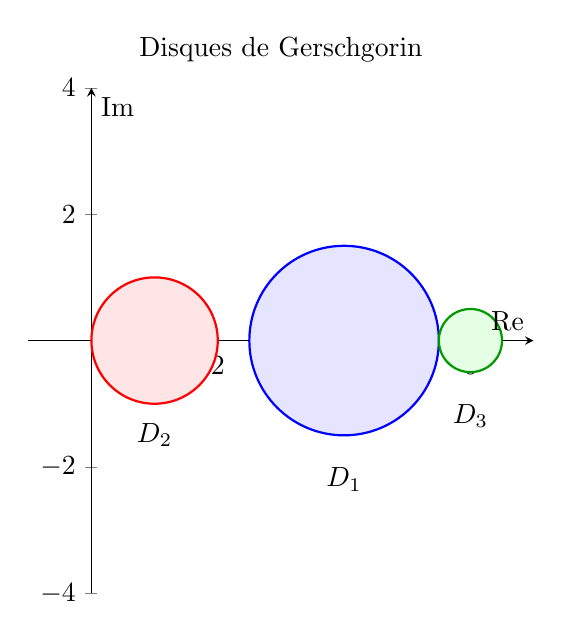
\begin{tikzpicture}
\begin{axis}[
  width=8cm, height=8cm, axis equal, axis lines=middle,
  xlabel={Re}, ylabel={Im}, xmin=-1, xmax=7, ymin=-4, ymax=4,
  title={Disques de Gerschgorin}
]
\draw[thick,blue,fill=blue!10] (axis cs:4,0) circle (1.5);
\draw[thick,red,fill=red!10] (axis cs:1,0) circle (1);
\draw[thick,green!60!black,fill=green!10] (axis cs:6,0) circle (0.5);
\node at (axis cs:4,-2.2) {$D_1$};
\node at (axis cs:1,-1.5) {$D_2$};
\node at (axis cs:6,-1.2) {$D_3$};
\end{axis}
\end{tikzpicture}
\end{center}

\section{Exemple num\'erique}

$A=\begin{pmatrix}4&1&0\\1&3&1\\0&1&2\end{pmatrix}$, valeurs propres exactes : $\lambda\approx 5{,}049$, $2{,}643$, $1{,}307$.

\begin{center}
\begin{tabular}{cccc}
\toprule
It\'eration $k$ & $\lambda_1^{(k)}$ & $\lambda_2^{(k)}$ & $\lambda_3^{(k)}$ \\
\midrule
0 (Puissance) & 4.000 & -- & -- \\
5 & 5.023 & -- & -- \\
10 & 5.048 & -- & -- \\
20 & 5.049 & -- & -- \\
\midrule
QR $k=5$ & 5.049 & 2.644 & 1.307 \\
QR $k=10$ & 5.049 & 2.643 & 1.307 \\
\bottomrule
\end{tabular}
\end{center}

\section{Impl\'ementation}

\begin{codeblock}[title=\textbf{Python}]
\begin{minted}{python}
import numpy as np

def power_iteration(A, x0=None, tol=1e-10, maxiter=1000):
    n = A.shape[0]
    x = x0 if x0 is not None else np.random.randn(n)
    x = x / np.linalg.norm(x)
    lam_old = 0
    for k in range(maxiter):
        w = A @ x
        x = w / np.linalg.norm(w)
        lam = x @ A @ x  # Rayleigh quotient
        if abs(lam - lam_old) < tol:
            break
        lam_old = lam
    return lam, x

def inverse_iteration(A, mu=0, x0=None, tol=1e-10, maxiter=1000):
    n = A.shape[0]
    x = x0 if x0 is not None else np.random.randn(n)
    x = x / np.linalg.norm(x)
    B = A - mu * np.eye(n)
    lu = np.linalg.lu_factor(B) if np.linalg.det(B) != 0 else None
    lam_old = 0
    for k in range(maxiter):
        if lu is not None:
            w = np.linalg.lu_solve(lu, x)
        else:
            w = np.linalg.solve(B, x)
        x = w / np.linalg.norm(w)
        lam = x @ A @ x
        if abs(lam - lam_old) < tol:
            break
        lam_old = lam
    return lam, x

def qr_algorithm(A, maxiter=100):
    Ak = A.astype(float).copy()
    n = Ak.shape[0]
    for k in range(maxiter):
        Q, R = np.linalg.qr(Ak)
        Ak = R @ Q
        # Check convergence (sub-diagonal elements)
        off = np.sum(np.abs(np.tril(Ak, -1)))
        if off < 1e-12:
            break
    return np.diag(Ak)

# Test
A = np.array([[4, 1, 0],
              [1, 3, 1],
              [0, 1, 2]], dtype=float)

lam1, v1 = power_iteration(A)
print(f"Puissance iteree: lambda_1 = {lam1:.6f}")
print(f"numpy.linalg.eig: {sorted(np.linalg.eig(A)[0], reverse=True)}")

eigenvalues_qr = qr_algorithm(A)
print(f"QR algorithm: {sorted(eigenvalues_qr, reverse=True)}")

# SVD
B = np.array([[1, 2], [3, 4], [5, 6]], dtype=float)
U, s, Vt = np.linalg.svd(B)
print(f"Valeurs singulieres: {s}")
print(f"cond(B) = {s[0]/s[-1]:.4f}")
\end{minted}
\end{codeblock}

\begin{codeblock}[title=\textbf{Julia}]
\begin{minted}{julia}
using LinearAlgebra

function power_iteration(A; x0=nothing, tol=1e-10, maxiter=1000)
    n = size(A, 1)
    x = x0 === nothing ? randn(n) : copy(x0)
    x ./= norm(x)
    lam_old = 0.0
    lam = 0.0
    for k in 1:maxiter
        w = A * x
        x = w / norm(w)
        lam = dot(x, A * x)
        abs(lam - lam_old) < tol && return lam, x
        lam_old = lam
    end
    return lam, x
end

function qr_algorithm(A; maxiter=100)
    Ak = float.(copy(A))
    for k in 1:maxiter
        Q, R = qr(Ak)
        Ak = R * Matrix(Q)
        sum(abs.(tril(Ak, -1))) < 1e-12 && break
    end
    return diag(Ak)
end

A = [4.0 1 0; 1 3 1; 0 1 2]
lam, v = power_iteration(A)
println("Puissance iteree: lambda_1 = $lam")
println("eigvals: $(eigvals(A))")
println("QR: $(sort(qr_algorithm(A), rev=true))")

# SVD
B = [1.0 2; 3 4; 5 6]
F = svd(B)
println("Valeurs singulieres: $(F.S)")
println("cond(B) = $(F.S[1]/F.S[end])")
\end{minted}
\end{codeblock}

\section{Exercices}

\begin{exercice}[$\star$]
Appliquer la m\'ethode de la puissance \`a $A=\begin{pmatrix}2&1\\1&3\end{pmatrix}$ avec $x^{(0)}=(1,1)^\top$. Calculer les 5 premi\`eres it\'erations.
\end{exercice}

\begin{exercice}[$\star\star$]
Montrer que l'it\'eration QR pr\'eserve la similarit\'e : $A_{k+1}=Q_k^\top A_k Q_k$.
\end{exercice}

\begin{exercice}[$\star\star$]
Tracer les disques de Gerschgorin pour $A=\begin{pmatrix}5&1&0\\1&3&0{,}5\\0&0{,}5&1\end{pmatrix}$ et localiser les valeurs propres.
\end{exercice}

\begin{exercice}[$\star\star\star$ -- Projet]
Impl\'ementer l'algorithme QR avec r\'eduction de Hessenberg et d\'ecalage de Wilkinson. Comparer les performances avec l'algorithme QR basique sur des matrices al\'eatoires de taille $n=50,100,200$.
\end{exercice}

\begin{formules}
\begin{align*}
Ax &= \lambda x, \quad \rho(A)=\max|\lambda_i| \\
\text{Puissance} &: x^{(k)}=\frac{Ax^{(k-1)}}{\|Ax^{(k-1)}\|}, \quad \BigO(|\lambda_2/\lambda_1|^k) \\
\text{QR} &: A_k=Q_kR_k,\; A_{k+1}=R_kQ_k \\
\text{SVD} &: A=U\Sigma V^\top, \quad \cond_2(A)=\sigma_1/\sigma_n
\end{align*}
\end{formules}
